\chap{ Switches, Lights, and Multiplexers}
\section{Part I }
\begin{itemize}
    \item [] \textbf{REQUIREMENT}
        \begin{enumerate}
            \item Create a new Quartus project for your circuit. Select the target chip that corresponds to your DE-series board. Refer to Table 1 for a list of devices.
            \item Create a Verilog module for the code in Figure 1 and include it in your project.
            \item Include in your project the required pin assignments for your DE-series board, as discussed above. Compile the project.
            \item Download the compiled circuit into the FPGA chip by using the Quartus Programmer tool (the procedure for using the Programmer tool is described in the tutorial Quartus Introduction). Test the functionality of the circuit by toggling the switches and observing the LEDs.
        \end{enumerate}
    \item [] \textbf{SOLUTION}
            \begin{lstlisting}[language=verilog]
module part2(out, X, Y,S);
    output	[3:0]out;
    input		[3:0]X,Y;
    input		S;
    
    assign out = ({4{S}}&X) | ({4{~S}}&Y);
endmodule
            \end{lstlisting}
             \begin{figure}[h]
                \centering
                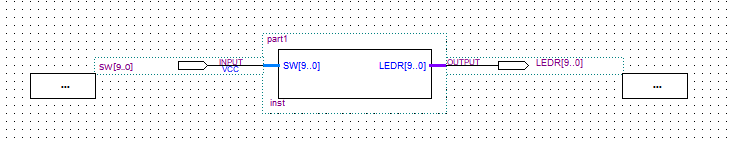
\includegraphics[scale = 0.9]{source/picture/Lab1/Lab1_1.png}
                \caption{Schematic for part 1}
            \end{figure}
\end{itemize}
\clearpage
\section{Part II }
\begin{itemize}
    \item [] \textbf{REQUIREMENT}
        \begin{enumerate}
            \item Create a new Quartus project for your circuit.
            \item Include your Verilog file for the four-bit wide 2-to-1 multiplexer in your project. Use switch $SW_9$ as the s input, switches $SW_{3-0}$ as the X input and $SW_{7-4}$ as the Y input. Display the value of the input s on $LEDR_9$, connect the output M to $LEDR_{3-0}$, and connect the unused LEDR lights to the constant value 0.
            \item Include in your project the required pin assignments for your DE-series board. As discussed in Part I, these assignments ensure that the ports of your Verilog code will use the pins on the FPGA chip that are connected to the SW switches and LEDR lights.
            \item Compile the project, and then download the resulting circuit into the FPGA chip. Test the functionality of the four-bit wide 2-to-1 multiplexer by toggling the switches and observing the LEDs
        \end{enumerate}
    \item [] \textbf{SOLUTION}
        \begin{lstlisting}[language= verilog]
module part2(out, X, Y,S);
	output	[3:0]out;
	input		[3:0]X,Y;
	input		S;
	
	assign out = ({4{S}}&X) | ({4{~S}}&Y);
	
endmodule
        \end{lstlisting}
        \begin{figure}[h]
            \centering
            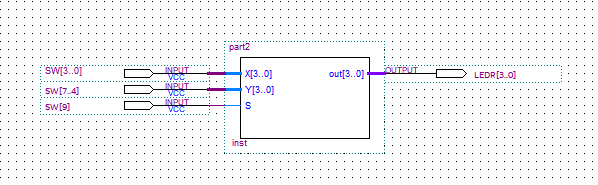
\includegraphics[scale =0.9]{source/picture/Lab1/Lab1_2.png}
            \caption{Schematic for part 2}
        \end{figure}
\end{itemize}
\clearpage
\section{Part III }
\begin{itemize}
    \item [] \textbf{REQUIREMENT}
        \begin{enumerate}
            \item Create a new Quartus project for your circuit.
            \item Create a Verilog module for the two-bit wide 4-to-1 multiplexer. Connect its select inputs to switches $SW_{9-8}$, and use switches $SW_{7-0}$ to provide the four 2-bit inputs U to X. Connect the output M to the red lights $LEDR_{1-0}$.
            \item Include in your project the required pin assignments for your DE-series board. Compile the project.
            \item Download the compiled circuit into the FPGA chip. Test the functionality of the two-bit wide 4-to-1 multiplexer by toggling the switches and observing the LEDs. Ensure that each of the inputs U to X can be properly selected as the output M.
        \end{enumerate}
    \item [] \textbf{SOLUTITON}
        \begin{lstlisting}[language = verilog]
module part3(M,U,V,W,X,S_1,S_0);
    input 	[1:0]U,V,W,X;
    input		S_1,S_0;
    output	[1:0]M;
    
    assign 	M= ({2{S_0&S_1}}&X)|
                    ({2{~S_0&S_1}}&W)|
                    ({2{S_0&~S_1}}&V)|
                    ({2{~S_0&~S_1}}&U);
	
endmodule
        \end{lstlisting}
        \begin{figure}[h]
            \centering
            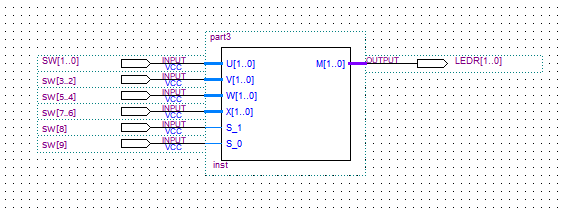
\includegraphics[width = \textwidth]{source/picture/Lab1/Lab1_3.png}
            \caption{Schemactic for part 3}
        \end{figure}
    
\end{itemize}
\clearpage
\section{Part IV }
\begin{itemize}
    \item [] \textbf{REQUIREMENT}
    \begin{enumerate}
        \item The objective of this part is to display a character on a 7-segment display. This decoder produces seven outputs that are used to display a character on a 7-segment display. Table 2 lists the characters that should be displayed for each valuation of c1c0 for your DE-series board.
        \item Note that in some cases the ‘blank’ character is selected for code 11. The seven segments in the display are identified by the indices 0 to 6 shown in the figure. Each segment is illuminated by driving it to the logic value 0. You are to write a Verilog module that implements logic functions to activate each of the seven segments.
    \end{enumerate}    
        \begin{figure}[h]
            \centering
            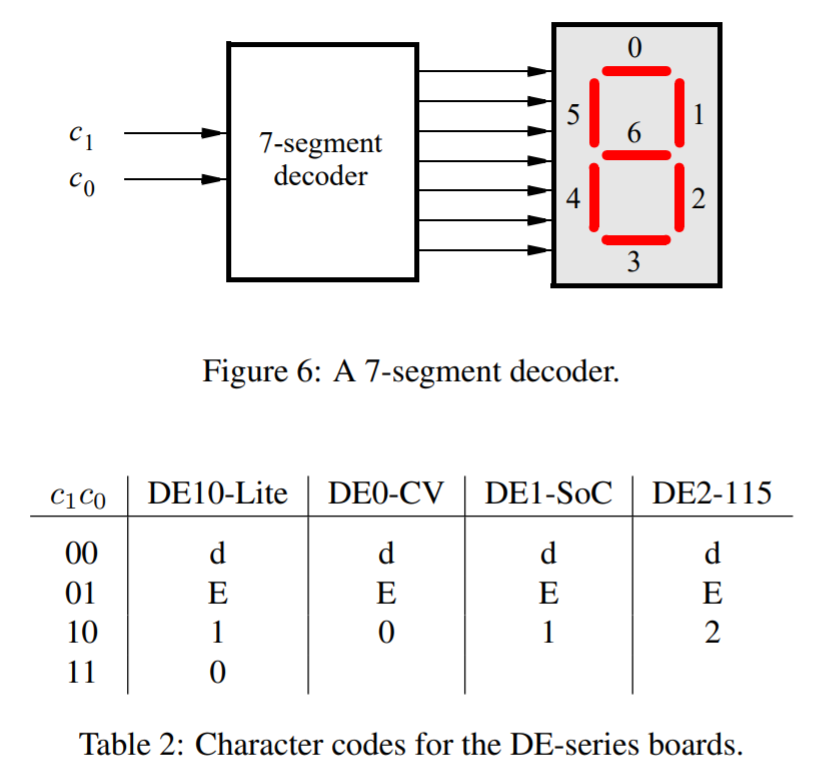
\includegraphics[scale =0.4]{source/picture/Lab1/1-4.png}
        \end{figure}
    \item [] \textbf{SOLUTION}
        \begin{lstlisting} [language = verilog]
module  part4(OUT,C_IN);
    input 	[1:0]C_IN;
    output	[6:0]OUT;
    
    assign 	OUT = (C_IN==0) ? 7'b0100001: 
                  (C_IN==1) ? 7'b0000110: 
                  (C_IN==2) ? 7'b0100100:7'b1111011;
endmodule
        \end{lstlisting}
        \begin{figure}[h]
            \centering
            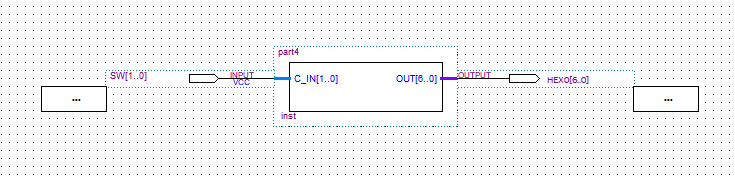
\includegraphics[width=\textwidth]{source/picture/Lab1/Lab1_4.png}
            \caption{Schemtatic for part 4}
        \end{figure}
\end{itemize}

\clearpage
\section{Part V }
\begin{itemize}
    \item [] \textbf{REQUIREMENT}
        \begin{enumerate}
            \item Consider the circuit shown in Figure 7. It uses a two-bit wide 4-to-1 multiplexer to enable the selection of four characters that are displayed on a 7-segment display. Using the 7-segment decoder from Part IV this circuit can display the characters d, E, 0, 1, 2, or 'blank' depending on your DE-series board. The character codes are set according to Table 2 by using the switches SW7-0, and a specific character is selected for display by setting the switches $SW_{9-8}$.
            \item Note that we have used the circuits from Parts III and IV as subcircuits in this code. The purpose of your circuit is to display any word on the four 7-segment displays that is composed of the characters in Table 2, and be able to rotate this word in a circular fashion across the displays when the switches SW9-8 are toggled. As an example, if the displayed word is dE10, then your circuit should produce the output patterns illustrated in Table 3.
        \end{enumerate}
        \begin{figure}[h]
            \centering
            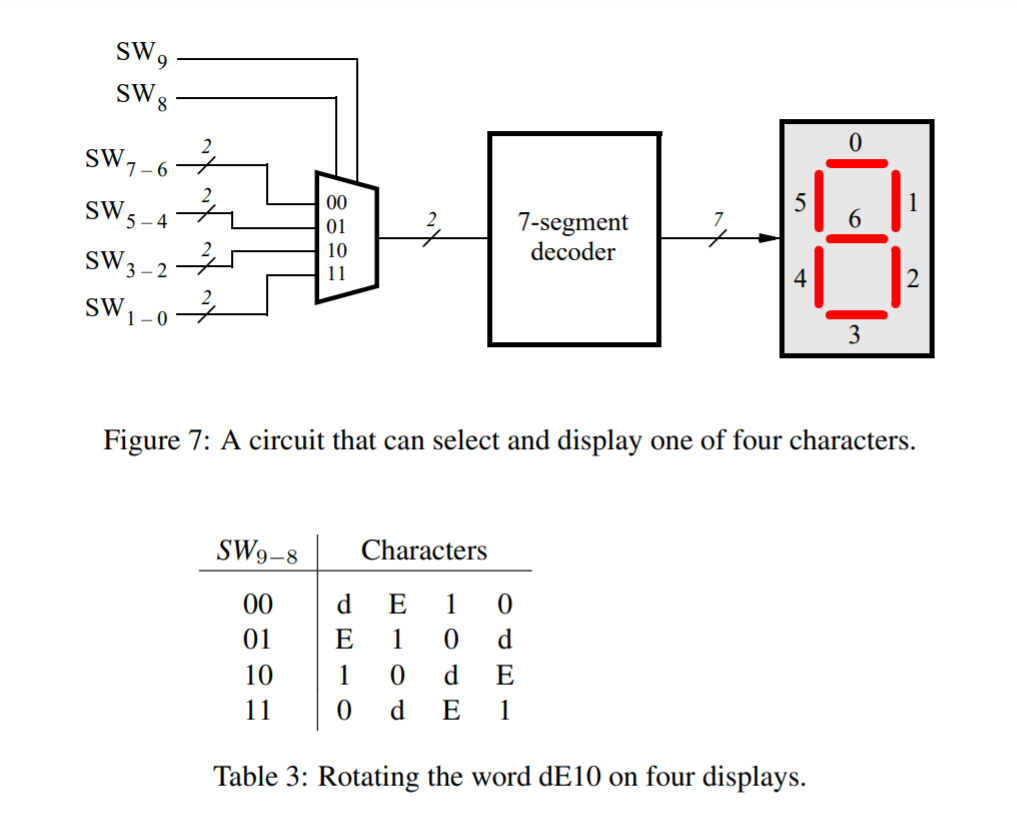
\includegraphics[scale =0.40]{source/picture/Lab1/1-5.png}
        \end{figure}
    \item [] \textbf{SOLUTION} In this part of Lab 1, we reuse part 3 and part 4  block to implement the circuit. 
        \begin{itemize}
            \item [] Part 3 block with 4 fix input and Pin $S_0, S_1$ to select the input
            \item [] Part 4 block use the output of the part 3 as the input and generate signal for four 7-segment leds in DE2i-board.
        \end{itemize}
         
\end{itemize}
\clearpage
\begin{figure}[h]
    \centering
    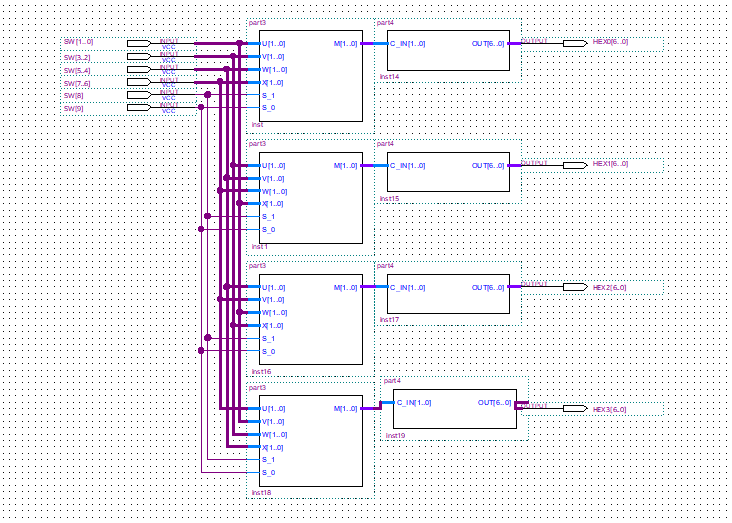
\includegraphics[width=\textwidth]{source/picture/Lab1/Lab1_5.png}
    \caption{Schematic for part 5}
\end{figure}
\clearpage

\section{Part VI }
\begin{itemize}
    \item [] \textbf{REQUIREMENT}
        \begin{enumerate}
            \item Extend your design from Part V so that is uses all 7-segment displays on your DE-series board. Your circuit needs to display a three- or four-letter word, corresponding to Table 2, using 'blank' characters for unused displays. Implement rotation of this word from right-to-left as indicated in Table 4 and Table 5. 
            \item Note that for the DE10-Lite you will need to use 3-bit codes for your characters, because five characters are needed when including the 'blank' character (your 7-segment decoder will have to use 3-bit codes, and you will need to use 3-bit wide 6-to-1 multiplexers). 
        \end{enumerate}
    \item [] \textbf{SOLUTION}
        \begin{lstlisting}[language=Verilog]
module part6(SW,HEX0, HEX1, HEX2, HEX3, HEX4, HEX5, HEX6, HEX7);
	input 	[2:0]SW;
	output 	[6:0]HEX0,HEX1,HEX2, HEX3, HEX4, HEX5, HEX6, HEX7;
	wire		[55:0]hex0,hex1,hex2,hex3,hex4,hex5,hex6,hex7;
	wire		[55:0]temp;

	assign hex0 = {7'b1111111,7'b1111111,7'b1111111,7'b1111111,7'b0100001,7'b0000110,7'b1111001,7'b1111111};
	assign hex1 = {7'b1111111,7'b1111111,7'b1111111,7'b0100001,7'b0000110,7'b1111001,7'b1111111,7'b1111111};
	assign hex2 = {7'b1111111,7'b1111111,7'b0100001,7'b0000110,7'b1111001,7'b1111111,7'b1111111,7'b1111111};
	assign hex3 = {7'b1111111,7'b0100001,7'b0000110,7'b1111001,7'b1111111,7'b1111111,7'b1111111,7'b1111111};
	assign hex4 = {7'b0100001,7'b0000110,7'b1111001,7'b1111111,7'b1111111,7'b1111111,7'b1111111,7'b1111111};
	assign hex5 = {7'b0000110,7'b1111001,7'b1111111,7'b1111111,7'b1111111,7'b1111111,7'b1111111,7'b0100001};
	assign hex6 = {7'b1111001,7'b1111111,7'b1111111,7'b1111111,7'b1111111,7'b1111111,7'b0100001,7'b0000110};
	assign hex7 = {7'b1111111,7'b1111111,7'b1111111,7'b1111111,7'b1111111,7'b0100001,7'b0000110,7'b1111001};
	
	assign temp = (SW==0)?hex0: 
					  (SW==1)?hex1:
					  (SW==2)?hex2:
					  (SW==3)?hex3:
					  (SW==4)?hex4:
					  (SW==5)?hex5:
					  (SW==6)?hex6:hex7;
					  
	assign HEX0 = temp[6:0];
	assign HEX1 = temp[13:7];
	assign HEX2 = temp[20:14];
	assign HEX3 = temp[27:21];
	assign HEX4 = temp[34:28];
	assign HEX5 = temp[41:35];
	assign HEX6 = temp[48:42];
	assign HEX7 = temp[55:49];
	
endmodule
    \end{lstlisting}
\end{itemize}

\clearpage



\begin{figure}[h]
    \centering
    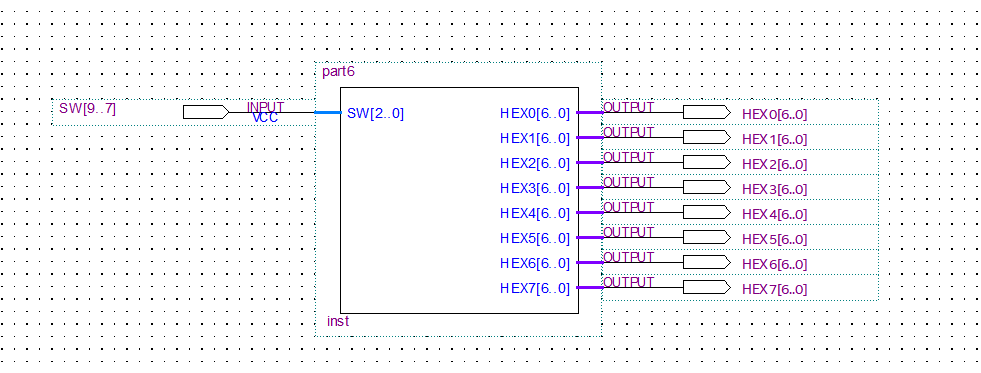
\includegraphics[width = \textwidth]{source/picture/Lab1/Lab1_6.png}
    \caption{Schematic for part 6}
\end{figure}

\begin{figure}[h]
    \centering
    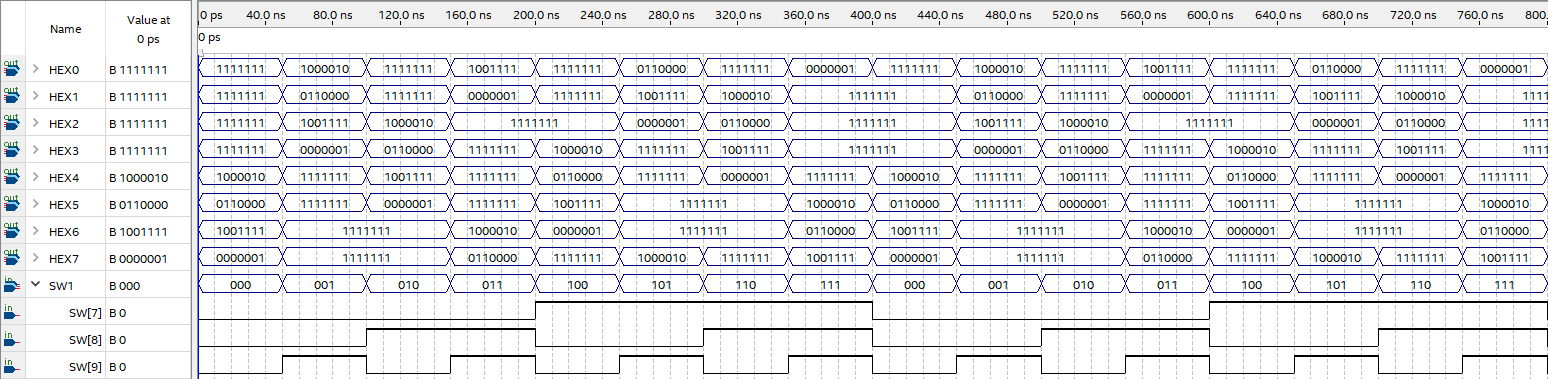
\includegraphics[scale = 0.40]{source/picture/Lab1/Lab1_wave.png}
    \caption{Simulation Result}
\end{figure}